\documentclass[11pt]{article}

\usepackage{microtype}
\usepackage{amsmath}
\usepackage{xcolor}
\usepackage{graphicx}
\usepackage{enumitem}


\setlength{\parindent}{0cm}
\renewcommand\thesubsection{\alph{subsection})}

\title{\textbf{Assignment 1\\}Search Algorithms}
\author{Malik Al-hallak 90020\\
		Sebastian Utzig 100059\\
		Clemens Wegener 91268}
\date{}
\begin{document}

\maketitle

\setcounter{section}{3} %counter manuell erhöhen
\section{Search Space}
The method \texttt{cleanup\_closed} removes nodes from the CLOSE list which are not part of the solution path. All dead end nodes fulfill this criterion, therefore the nodes \emph{k} and \emph{u} are deleted. Furthermore, all predecessors of the deleted dead end nodes which don't have successors on the OPEN list, and therefore cannot be part of the solution path, can be deleted. Node \emph{c} fulfills this and hence is deleted too.


\begin{figure}[ht]
	\centering
  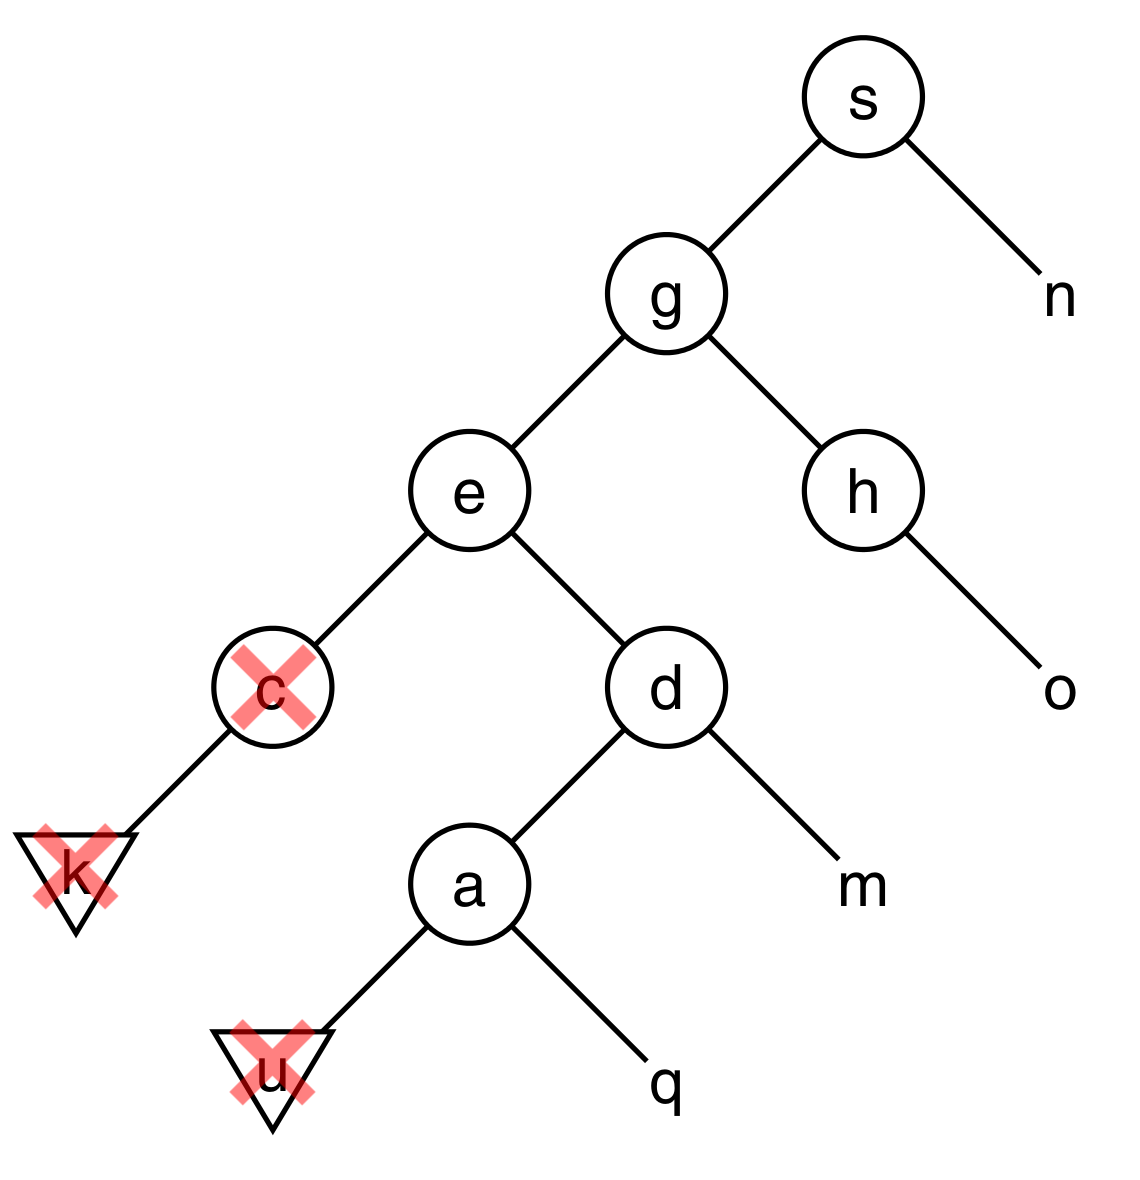
\includegraphics[width=0.5\textwidth]{./graph_7.png}
  \caption{Graph after \texttt{cleanup\_closed}}
	\label{fig2}
\end{figure}

\setcounter{section}{6}
\section{Hill-Climbing}

\begin{minipage}{0.5\textwidth}
	\subsection{}
	\begin{align*}
		n=s=0\\
		n_{opt}=s=0\\\\
		n_{opt}=2\\
		n_{opt}=3\\\\
		n_{opt}=4\\
		n_{opt}=6\\\\
		n_{opt}=7^*\\
		n_{opt}=8^*\\\\
		return\hspace{0.3cm}n_{opt}=8^*
	\end{align*}
\end{minipage}
\begin{minipage}{0.5\textwidth}
	\subsection{}
	\begin{align*}
		n=s=0\\
		n_{opt}=s=0\\\\
		n_{opt}=1\\
		n_{opt}=3\\\\
		n_{opt}=2\\
		n_{opt}=5\\\\
		n_{opt}=6\\\\\\
		return\hspace{0.3cm}Fail
	\end{align*}
\end{minipage}


\end{document}
